%!TEX root = main.tex

\section{Data and Experiments}
\label{sec:experiments}
%%In this section, 
We now evaluate our strategies for drivers 
in practice. First, we discuss how we collect and combine the appropriate data 
from multiple data sources. Then, we perform a comprehensive experimental study
%that reveals the benefits of being strategic for the drivers and 
that provides
specific insights as to how NYC drivers can maximize their earnings.

\subsection{Data collection and preparation}
In order to evaluate our strategies, we need to construct 
time-evolving matrices 
{\empiricaltransitionmatrix}, {\traveltimematrix} and {\rewardsmatrix} as defined in Section~\ref{sec:problem_setup},
and {\countmatrix} as defined in Section~\ref{sec:sensitivity}.
For this, we use two data sources: (1) the NYC taxi rides 
dataset\footnote{\url{http://www.nyc.gov/html/tlc/html/about/trip_record_data.shtml}} and
(2) information we obtain from the Uber platform via queries to the Uber API.\footnote{\url{https://developer.uber.com/docs/riders/ride-requests/tutorials/api/introduction}}

\begin{figure}
	\centering
	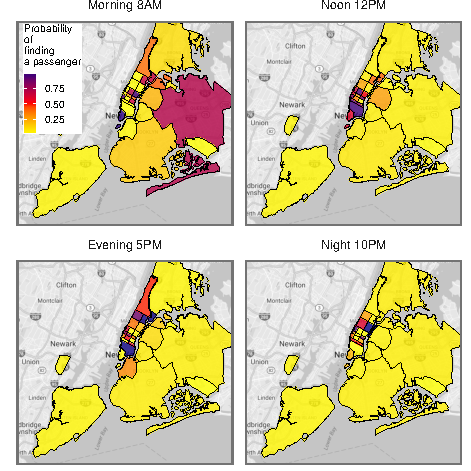
\includegraphics{figures/successful_heatmap.pdf}
	\setlength{\belowcaptionskip}{-10pt}
	\caption{Probability of finding a passenger in 10 minutes across NYC zones at different times of a representative day.}
	\label{fig:successful_heatmap}
\end{figure}


\spara{Forming time-evolving matrices {\countmatrix} and {\empiricaltransitionmatrix}:}
Our starting point is the NYC Taxi  dataset (2015-2016), which
%%\footnote{\url{http://www.nyc.gov/html/tlc/html/about/trip_record_data.shtml}}. 
contains yellow street-hail records of over 200,000 taxi rides per day with fields capturing pickup and dropoff times, 
location co-ordinates, trip distances, and fares.
Each taxi record is accompanied with a taxi location ID for the pick-up and drop-off locations. 
Each location ID is associated with one of 29 non-overlapping city zones, as defined in the
dataset.  While the set of taxi rides is undoubtedly produced from a different ridership than Uber, 
%resulting in differences of geographical diversity, demographics, and timing, 
it nonetheless provides a useful baseline that reflects many of the broader dynamics of ridership demand in 
NYC. %over space and time.  %Thus we this to build count and frequency input matrices, as follows.


Given this data, we divide each 24-hour day of the week into 144 time-slices of duration 10 minutes each, indexed by their start 
time.  To model traffic demand in the city at time $t$, the $c(i,j)$ entry of count matrix $\countmatrix^t$ is the total 
number of rides from zone $i$ to zone $j$ in a 30-minute long time window centered at time $t$. For example, 
$c(i,j)$ for the time slot [10:40, 10:50] on a Wednesday is a count of all rides 
from $i$ to $j$ that were initiated between 10:30 and 11:00 
on {\em{any}} Wednesday in the dataset. 
Since our model disallows rides within the same zone, we ignore such rides while populating the entries of 
  the matrix $\countmatrix^t$, resulting in all diagonal entries of the count matrix being zero.

%% Every diagonal entry of the count matrix $\countmatrix^t$ is zero.
%%However, the empirical transition matrix $\empiricaltransitionmatrix^t$ described in Section \ref{sec:problem_setup} assumes that the diagonal entries $f^t(i,i)$ denote the probabilities of a driver not finding a passenger in zone $i$ in the time-slice $t$. We compute these probabilities below.

To populate the entries of the empirical transition matrix $\empiricaltransitionmatrix^t$, as 
  defined in Section \ref{sec:problem_setup}, we must estimate its diagonal entries, 
  which correspond to the probability of not finding a ride, as well as the transition probabilities.
We derive these from the data as follows.
%\spara{Modeling successful passenger pickup}:
Assuming that the parameters do not change significantly within a single time-slice, let $N(\passengerarrivalrate)$ and $N(\driverarrivalrate)$ denote the number of passenger and driver arrivals in zone $i$ in one time unit, with 
independent\footnote{Although we assume the independence of the passenger and driver arrival processes, we can also accommodate correlated processes with slight modification.} Poisson arrival rates {\passengerarrivalrate} and {\driverarrivalrate} respectively. Hence, the random variable $K = N(\passengerarrivalrate) - N(\driverarrivalrate)$ follows a Skellam distribution
such that:
\begin{equation*}
\Pr[K=k] = e^{-(\passengerarrivalrate + \driverarrivalrate)} \bigg(\frac{\passengerarrivalrate}{\driverarrivalrate}\bigg) I_k\big(2 \sqrt{\passengerarrivalrate \driverarrivalrate}\big)
\end{equation*}
where $I_k(z)$ is the modified Bessel function of the first kind~\cite{wiki:skellam}. 

Whenever %the Markov Chain is in a non-positive state, 
$K<0$, there are more drivers than passengers. We assume a worst case scenario in which a driver (conceptually) joins the end
 of a FIFO queue for that zone. Hence, for $k \leq 0$, the driver has to wait for $(|k| + 1)$ passenger arrivals for a successful passenger pickup. Then, the probability of a successful passenger pickup is:
\begin{equation*}
\Pr[N(\passengerarrivalrate) = |k| + 1] = \frac{\passengerarrivalrate^{\big(|k|+1\big)} e^{-\passengerarrivalrate}}{\big(|k| + 1\big)!}.
\end{equation*}
Thus, we can express a diagonal entry $f^t(i,i)$ as follows:
\begin{equation*}
f^t(i,i) = 1 - \sum_{k \leq 0} \Pr[K = k] \times \Pr[N(\passengerarrivalrate) \geq |k| + 1].
\end{equation*}
For {\empiricaltransitionmatrix} to be stochastic, we set every other entry 
$f^t(i,j)$ to:
\begin{equation*}
f^t(i,j) = (1 - f^t(i,i)) \times \frac{c^t(i,j)}{\sum_{j}c^t(i,j)}. 
\end{equation*}
The matrix $\empiricaltransitionmatrix^t$ built in this manner satisfies all our assumptions. %and can be used as input to our algorithms. 

Figure \ref{fig:successful_heatmap} shows an example of varying estimated probabilities of successful pickups 
  in different zones at various times of the day derived from the NYC data using the methods above. 
As expected, we see that the probability of a successful pickup is higher outside Manhattan in the morning, 
  and this trend reverses in the evening.

\begin{figure*}
	\centering
	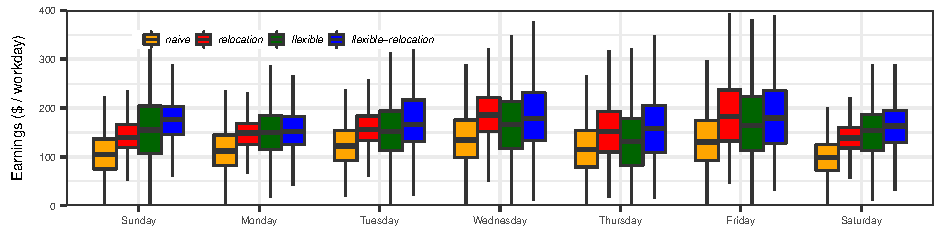
\includegraphics{figures/daily_simulated_earnings.pdf}
	\setlength{\belowcaptionskip}{-5pt}
	\caption{Daily driver earnings for different strategies averaged over different home zones on a representative day.}
	\label{fig:daily_earnings}
\end{figure*}

\spara{Forming time-evolving matrices {\traveltimematrix} and {\rewardsmatrix}:} We obtain information regarding travel times and rewards using the \texttt{estimates/price} endpoint of the Uber API.
The API takes longitude and latitude of pick-up and drop-off locations and returns price estimates for all types of Uber products -- UberX, UberXL and UberBlack --  together with the active surge multiplier rate at the pick-up location at the time of query.  We only focus on UberX, the most popular Uber product. We also use the \texttt{/products} API endpoint to get information on the base fare, minimum fare, cost per minute and cost per unit distance for UberX. However, none of the Uber API endpoints provide information about the supply of  drivers or demand of passengers; we impute this 
information from the NYC taxi rides dataset.

To create a representative sample of the data, we ``recreated'' NYC taxi rides virtually on the Uber platform. 
Using the Uber API, we were able to take a NYC taxi ride recorded in 2015, and capture the Uber attributes of that ride exactly 
one year later, collecting price estimates and other data above for that virtual ride.
To respect the Uber rate limit of 1,000 API requests per hour per account, we sub-sampled one ride between each pair of zones in
the city every 15 minutes.
% (if such a ride occurred in the taxi dataset).
We implicitly assume that price estimates, travel times, and distance of preferred travel paths by drivers do not vary 
significantly in 15 minutes. Every 5 minutes, we also queried the surge multiplier active within each zone.\footnote{Chen {\etal}~\cite{chen2015peeking} have observed that 90\% of the surges on Uber platform 
have durations lasting multiples of 5 minutes.} 
Using this approach, we collected data from the Uber API for a 6-month period (Oct. 2016--Mar 2017), 
recreating rides that originally occurred from 
Oct. 2015 to Mar 2016.   Thus, we built realistic estimates for $r(i,j)$ and $\tau(i,j)$
for all pairs of zones\footnote{We take into account the Uber fee structure in NYC as reported by the Uber API, as well as the overall \emph{cost per mile} estimates provided by the American Automobile Association (AAA) in order to build realistic estimates for $r(i,j).$}.  Finally, we maintained same-day of week estimates, so that, for example, travel time estimates
and rewards computed for Sunday, Oct 16, 2016, were paired with frequency estimates drawn from the NYC taxi rides dataset for
Sunday, Oct. 18, 2015.
%However, due to seasonality of the data, 
In the remainder of this section, we provide  results for driving during one representative week in October.
%starting on Sunday, October 18, 2015\footnote{In order to maintain uniformity of the day of the week between the NYC taxi rides dataset (2015) and the Uber data (2016), we use the Uber API data for the week starting on Sunday, October 16, 2016 to form the matrices {\traveltimematrix}, {\rewardsmatrix}. 
Our results do not vary qualitatively across different weeks, with the exception of seasonal peak days, such as New Year's Eve. 

%Although the \texttt{estimates/time} endpoint of the Uber API returns the estimated waiting time for a passenger at a particular location, it provides no information on the supply of UberX cars in its neighborhood. Consequently, we do not possess an exact estimate of the time spent by an Uber driver waiting for a passenger in a particular zone. 
%%endpoint to query rides from exact same pick-up to drop-off locations at the exact same time of the 
%%day on the same calendar date, but one year later.
%% i.e, a real recorded ride from November 10, 2015 was virtually recreated on November 10, 2016. 
%%However, Uber imposes a rate limit of 1,000 API requests per hour per account. To respect these API limits, we randomly sample rides between each pair of zones in the city every 15 minutes. 
%In the next section we discuss how we get an estimate of that quantity.
%
%However, in the next section, we provide a methodology to compute a conservative estimate of the driver waiting time in a particular zone at any time of the day using the successful passenger pick-up information from the NYC taxi rides dataset.

%However, due to seasonality of the data, we provide experimental results for one week starting on Sunday, October 18, 2015\footnote{In order to maintain uniformity of the day of the week between the NYC taxi rides dataset (2015) and the Uber data (2016), we use the Uber API data for the week starting on Sunday, October 16, 2016 to form the matrices {\traveltimematrix}, {\rewardsmatrix}. Our results do not vary qualitatively across different weeks or different days of the same week.}. 


%Using the same time-slicing as we described in the previous paragraph and the same
%29 city zones, the
%travel time matrix $\traveltimematrix^t$ and rewards matrix $\rewardsmatrix^t$ entries contain the average travel times and average rewards of traveling between two zones
%as computed by the above data-collection process. Note that each entry of the {\rewardsmatrix} matrix represents net reward, calculated after taking into account the surge information, along with driver expenses and Uber's share. %of earnings.


% \iffalse
% \subsection{Data collection}
% \label{sec:data}
% To evaluate our methods, we need a representative sample of taxi rides data. To obtain this data, we strategically sample rides from the publicly available NYC taxi rides 
% dataset~\footnote{\url{http://www.nyc.gov/html/tlc/html/about/trip_record_data.shtml}} and recreate them on the Uber platform using Uber API queries.

% \spara{The Uber API}: 
% The HTTP-based Uber API allows third-party developers to retrieve information about Uber. For our study, the most relevant endpoint of the API is \texttt{estimates/price}. It takes longitude and latitude of pick-up and drop-off locations and returns price estimates for all types of Uber products - UberX, UberXL and UberBlack. Along with the price estimates, it also provides the active surge multiplier rate at the pick-up location at the time of query. For the purpose of this study, we only focus on UberX, the most popular Uber product. We also use the \texttt{/products} endpoint to get information regarding the base fare, minimum fare, cost per minute and cost per unit distance for UberX. However, none of the Uber API endpoints provide information about the supply of UberX drivers or demand of passengers. To overcome this obstacle, we leverage the NYC taxi rides dataset.

% \spara{NYC taxi-rides dataset}:
% NYC taxi rides dataset\footnote{\url{http://www.nyc.gov/html/tlc/html/about/trip_record_data.shtml}} for the year 2015 contains yellow street-hail taxi records with fields capturing pick-up and drop-off dates/times, location co-ordinates, trip distances and fares. Each taxi record is accompanied with taxi location ID for the pick-up and drop-off locations. We use these location IDs to divide the city into a set of 29 non-overlapping zones.

% \spara{Querying the Uber API}:
% To create a representative sample of data, our strategy relies on `recreating' NYC taxi rides virtually on the Uber platform. We use the price estimates endpoint to query rides from exact same pick-up to drop-off locations at exact same time of the day on same calendar date, but exactly one year later i.e, a real recorded ride from 2015 is virtually recreated in 2016. However, Uber imposes a rate limit of 1,000 API requests per hour per account. To respect these API limits, we randomly sample rides between each pair of zones in the city every 15 minutes. We assume that price estimates, travel times and distance of preferred travel paths by drivers do not vary significantly in 15 minutes. Chen {\etal}~\cite{chen2015peeking} have observed that 90\% of the surges on Uber platform have durations as multiples of 5 minutes. Hence, every 5 minutes, we also query the surge multiplier active within each zone.

% Although the \texttt{estimates/time} endpoint of the Uber API returns the estimated waiting time for a passenger at a particular location, it provides no information on the supply of UberX cars in its neighborhood. Consequently, we do not possess an exact estimate of the time spent by an Uber driver waiting for a passenger in a particular zone. 
% In the next section we discuss how we get an estimate of that quantity.
% %
% %However, in the next section, we provide a methodology to compute a conservative estimate of the driver waiting time in a particular zone at any time of the day using the successful passenger pick-up information from the NYC taxi rides dataset.

% Using aforementioned approach, we collected data for a period of 6 months, recreating rides from October, 2015 till March, 2016. However, due to the periodicity of the data, we provide experimental results for one week starting October 18, 2015\footnote{Our results do not vary qualitatively across different weeks.}.

% \subsection{Experimental setup}
% In this section, we describe how the collected data can be used for modeling the dynamics of the city as well as an individual driver, as described in Section \ref{sec:problem_setup}.


% \spara{Modeling the city}:
% We divide each 24-hour day of the week in 144 time-slices of duration 10 minutes each, indexed by their start time. While modeling the city, the $c(i,j)$ entry of the count matrix $\countmatrix^t$ is the total number of rides from zone $i$ to zone $j$ in a 30-minute long time window centered around time $t$. 

% \begin{figure}
% 	\centering
% 	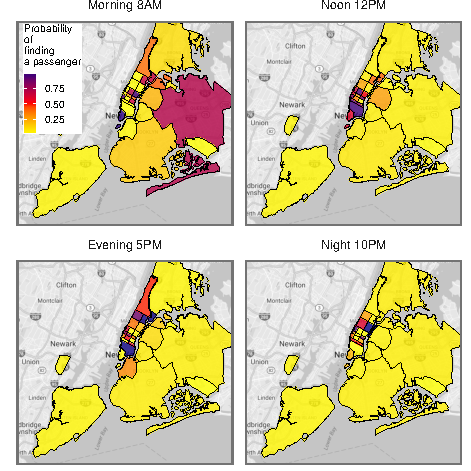
\includegraphics{figures/successful_heatmap.pdf}
% 	\caption{Estimated probability of finding a passenger within 10 minutes across NYC zones at different times of a representative day.}
% 	\label{fig:successful_heatmap}
% \end{figure}

% Similarly, travel time matrix $\traveltimematrix^t$ and rewards matrix $\rewardsmatrix^t$ entries contain the average travel times and average rewards of traveling between two zones. Recall that each entry of the {\rewardsmatrix} matrix represents the net reward, calculated after taking into account the surge multiplier, estimated driver expenses and Uber's share of the earnings.



% Now, we describe the formation of the empirical transition matrix $\empiricaltransitionmatrix^t$. Every diagonal entry of the count matrix $\countmatrix^t$ is zero, as there are no passenger rides within same zone. However, the empirical transition matrix $\empiricaltransitionmatrix^t$ described in Section \ref{sec:problem_setup} assumes that the diagonal entries $f(i,i)$ denote the probabilities of a driver not finding a passenger in zone $i$ in the time-slice $t$. Hence, to form the empirical transition matrix, we first normalize the observed count matrix such that each of its rows sum up to 1 and call this matrix $\countmatrix^\prime$. 
% In the following section, we describe the formation of empirical transition matrix $\empiricaltransitionmatrix^t$, using the matrix $\countmatrix^\prime$.

% %\spara{Modeling successful passenger pickup}:
% Let $N(\passengerarrivalrate)$ and $N(\driverarrivalrate)$ denote the number of passenger and driver arrivals in zone $i$ in one time unit, with Poisson arrival rates {\passengerarrivalrate} and {\driverarrivalrate} respectively. Assuming that passenger and driver arrivals are independent Poisson processes, the random variable $K = N(\passengerarrivalrate) - N(\driverarrivalrate)$ follows a Skellam distribution 
% %and can be depicted by states of a Markov Chain 
% such that:
% \begin{equation}
% \Pr[K=k] = e^{-(\passengerarrivalrate + \driverarrivalrate)} \bigg(\frac{\passengerarrivalrate}{\driverarrivalrate}\bigg) I_k\big(2 \sqrt{\passengerarrivalrate \driverarrivalrate}\big)
% \end{equation}
% where $I_k(z)$ is the modified Bessel function of the first kind\footnote{Although, for simplicity, we assume the independence of the passenger and driver arrival processes, we can also accommodate correlated processes with slight modification.}.

% Whenever %the Markov Chain is in a non-positive state, 
% $K<0$, there are more drivers than passengers in a given zone. We assume the worst case scenario in which a driver joins the corresponding FIFO queue at the last spot. Hence, for $k \leq 0$, the driver has to wait for $(|k| + 1)$ passenger arrivals for a successful passenger pickup. Then, the probability of a successful passenger pickup is:
% \begin{equation}
% \Pr[N(\passengerarrivalrate) = |k| + 1] = \frac{\passengerarrivalrate^{\big(|k|+1\big)} e^{-\passengerarrivalrate}}{\big(|k| + 1\big)!}
% \end{equation}
% Thus, we can express a diagonal entry $f(i,i)$ of empirical transition matrix as follows,
% \begin{equation}
% f(i,i) = 1 - \sum_{k \leq 0} \Pr[K = k] \times \Pr[N(\passengerarrivalrate) \geq |k| + 1]
% \end{equation}
% To maintain the right stochasticity of {\empiricaltransitionmatrix}, every other entry $f(i,j)$ is calculated as,
% \begin{equation}
% f(i,j) = (1 - f(i,i)) \times c^\prime(i,j)
% \end{equation}
% The matrix $\empiricaltransitionmatrix^t$, built in this manner satisfies all our assumptions and can be used in the evaluation of strategies described in previous sections. 

% Figure \ref{fig:successful_heatmap} shows an example of varying probabilities of successful pickups in different zones at various times of the day. As expected, we see that the probability of a successful pickup is higher outside Manhattan in the morning, and this trend reverses in the evening.

% \fi

\subsection{Experimental results}

% \begin{figure}
% 	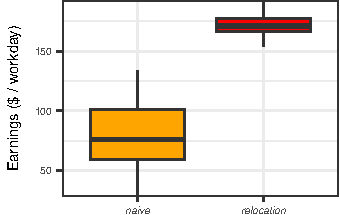
\includegraphics{figures/earnings_heatmap.pdf}
% 	\caption{Earnings from {\naive} and {\relocation} strategies for drivers across multiple 8-hour shifts starting from different home zones on a representative day.}
% 	\label{fig:earnings_heatmap}
% \end{figure}

\begin{figure*}     
	\centering
	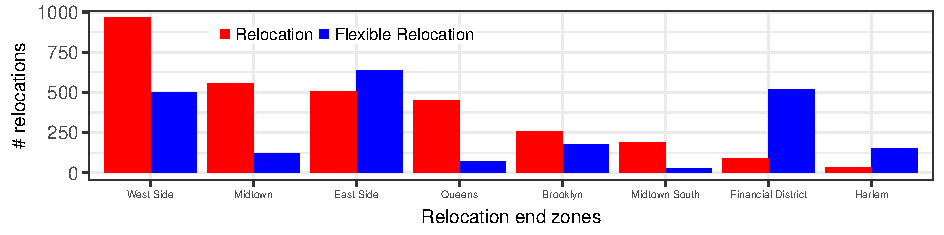
\includegraphics{figures/relocation_endzones.pdf}
	\setlength{\belowcaptionskip}{-5pt}
	\caption{Contrast between preferred relocation destinations for
	drivers with {\relocation} and {\relocationflexible} strategies
	on a representative day.}     
	\label{fig:relocation_endzones}
\end{figure*}

\begin{figure}[h]
	\centering
	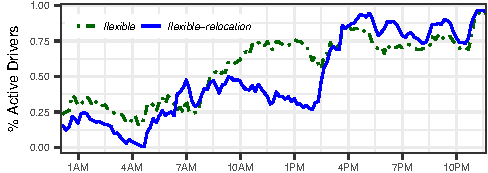
\includegraphics{figures/simulated_schedules.pdf}
	\setlength{\belowcaptionskip}{-10pt}
	\caption{Active drivers with {\flexible} and {\relocationflexible}
	strategies at different times of a representative day.}
	\label{fig:simulated_schedules}
\end{figure}

%Here, we evaluate our methodology. 
For all our experiments we use a single process implementation of our algorithms on a 24-core 2.9GHz Intel Xeon E5 processor with 512GB memory. Running time for  {\naive} and {\relocation}  is less than a minute, and about 5 minutes for  {\flexible} and  {\relocationflexible}. 
Uncertainty analysis (Section \ref{sec:effect_of_uncertainty}) with an off-the-shelf minimizer takes around 3 hours.

\spara{Comparison of strategies}: First, we address the question: \textit{what is the best driver strategy?} Intuitively, it is clear that {\relocationflexible} is the best strategy, as it takes advantage of spatial as well as temporal variations in the passenger demand across NYC. In order to verify this intuition, we compare driver earnings across different strategies. Drivers following the {\naive} and the {\relocation} strategies are assumed to drive from 9 AM to 5 PM, a standard 8 hour workday, while those following the {\flexible} or the {\relocationflexible} strategies drive for a total of 8 hours each day with a flexible schedule.

% Figure \ref{fig:daily_earnings} shows the average earnings achieved by 
% the solution to {\originalproblem} by each of the strategies on different days of a representative week. 
In order to evaluate the performance of our strategies, we find the solution to {\originalproblem} and simulate 100 drivers, each randomly assigned a 
home zone, operating on these strategies on the same day of the following week, for a total of 10 weeks. Figure \ref{fig:daily_earnings} presents a box-plot of the resulting earnings.\footnote{The lower and upper edges of the boxes in Figure \ref{fig:daily_earnings} indicate quartiles Q1 and Q3 respectively, and length of whisker is 1.5 times IQR.}.

We observe that all ``smart'' strategies consistently outperform {\naive};
as expected. On most days, {\relocationflexible} is the strategy with the highest earnings.
The median earning of a driver following the {\naive} strategy on a Sunday is \$104 while that of a driver following {\relocationflexible} is \$177, representing a 70\% increase in median earnings. 
Averaged over all days of the week, this results into a 47\% increase in median earnings per work day when following the {\relocationflexible} strategy. 
Thus, our strategies do exploit the spatial and the temporal variation in demand across NYC. The results also show
that for a part-time Uber driver in NYC, it is more beneficial to drive midweek, from Wednesday to Friday, and Sunday
than during Saturday and Monday.

%Having established that the {\relocation}, {\flexible} and {\relocationflexible} strategies result in higher driver earnings than the {\naive} strategy, in the subsequent sections, we further analyze various aspects related to them.

\spara{Spatial dynamics of strategies}: 
Next, we address the question - \textit{what are the benefits of the {\relocate} action?} Figure \ref{fig:successful_heatmap} already shows the spatial variation in the demand across different NYC zones at different times of the day.
Intuitively, this spatial variation can cause a disparity in the driver earnings based upon the zone of the driver. For example, drivers based in Manhattan should be expected 
to earn more than those based in Brooklyn due to persistently higher demand in Manhattan. Similarly, Figure \ref{fig:daily_earnings} shows temporal variation in earnings across days of the week. We observe that on the days of low-demand,
%%, especially on weekends, 
not only are the median earnings for {\relocation} consistently higher than those for {\naive} but also the inter-quartile range (IQR) and the length of whiskers for {\relocation} are narrower. On days with high but localized demand like Fridays, the {\relocation} strategy performs on par with the {\relocationflexible} strategy and significantly outperforms {\naive}.
% However, even
% at different times of the same day, drivers located within different parts of Manhattan itself will earn different amounts, 
% on account of temporal trends.
% Hence, instead of concentrating on the average earnings across different zones in a typical 9-5 workday from Figure \ref{fig:daily_earnings}, now we explore
% the variation in earnings of drivers starting from different home zones at different times of the day.


% The {\relocation} strategy attempts to mitigate the location-based disparity in earnings by suggesting optimal relocation actions to drivers at various times of the day. Figure \ref{fig:earnings_heatmap} shows variation in earnings from 8-hour driving shifts starting morning 8 AM, noon 12 PM, evening 5 PM and night 10 PM, for drivers with different home zones.
% Note that Figure~\ref{fig:earnings_heatmap} depicts the median earnings, as opposed to mean earnings shown in Figure~\ref{fig:daily_earnings}. Moreover, Figure~\ref{fig:earnings_heatmap} contains earnings from driving late-night shifts, which brings the median much lower.
% %Note that, on account of low earnings during shifts starting at noon and night, the median earnings in Figure \ref{fig:earnings_heatmap} are significantly lower than the mean earnings in Figure \ref{fig:daily_earnings}.
% Furthermore, not only do we observe that  {\relocation} has a higher median than the {\naive}, but also, the inter-quartile range (IQR) is significantly narrower.

These observations indicates that the location-based disparity in earnings for the {\naive} strategy is much larger than the {\relocation} strategy. Thus, we conclude that smart relocations throughout the day prevent a driver from becoming ``trapped'' in low-earning neighborhoods, translating 
into significant increases in the earnings. 
This may be counterintuitive to some drivers, as a {\relocate} action (essentially an empty ride) 
incurs cost to the driver. Yet, the results demonstrate that these actions, when timed appropriately, 
lead to earnings far higher than the costs they incur.


\spara{Temporal dynamics of strategies}: Intuitively, due to the periodicity of demand, we expect driver earnings to strongly depend on the time of the day they are driving. 
%We have also established via Figure \ref{fig:daily_earnings} that both of the flexible schedule strategies outperform their fixed schedule counterparts. 
Thus, we address the question: \textit{what is the best time of the day to drive in order to maximize earnings?} To answer this, we simulate 1000 drivers, each randomly assigned a home zone, for each of the {\flexible} and {\relocationflexible} strategies. 
We solve the {\originalproblem} problem for both strategies and create a recommended plan of action for the simulated drivers. 
Then, at every step of the simulation, a driver undertakes the personalized action recommended by the strategy, corresponding to
  their location, the time of day and their budget remaining.


In Figure \ref{fig:simulated_schedules}, we plot the percentage of simulated drivers driving in the city at different times of the day. We observe a noticeable difference between the ``preferred'' driving schedules 
output by {\flexible} and {\relocationflexible}.
In particular, a high percentage of {\flexible} schedule drivers are active during the standard working hours of the day from 9AM to 6PM. This also 
supports our choice to evaluate fixed schedule strategies in the interval 9AM to 5PM. In contrast, the number of active
drivers that follow {\relocationflexible} exhibits two distinct peaks, corresponding to the morning and the evening rush hours. Furthermore, over 50\% of {\relocationflexible} drivers use their driving budget in the latter half of the day starting approximately at 3PM, continuing through till midnight. 
Since {\flexible} and {\relocationflexible} only differ in 
the {\relocate} action, all observed differences are due to this action.
Hence, we can  conclude that the {\relocate} action is most effective in the evening hours, thereby prompting higher active percentages of {\relocationflexible} drivers at that time.

\spara{Preferred relocation zones}: By simulating drivers, we can also compare the {\relocate} actions between drivers 
following the {\relocation} strategy and those following the {\relocationflexible} strategy. 
The contrast between popular destinations 
of {\relocate} actions for drivers following the two strategies can be seen in Figure \ref{fig:relocation_endzones}. 
%We observe a contrast between the preferred relocation zones for drivers of these two strategies. 
Drivers following the {\relocation} strategy predominantly relocate themselves to the center of Manhattan. In contrast, the drivers following the {\relocationflexible} strategy do not exhibit a clear most-preferred relocation destination. Furthermore, the 
{\em number} of relocations performed by the {\relocation} strategy drivers, 
is, surprisingly, significantly higher than those performed by the {\relocationflexible} strategy drivers. 
This is due to the flexible work schedule of the latter, which allows them to drive 
  continuously during the hours of highest demand, reducing the frequency of {\relocate} actions they take. 

\subsection{Surge chasing}
\begin{figure}
	\centering
	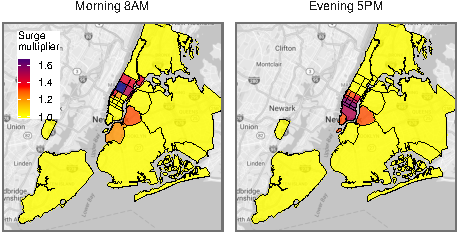
\includegraphics{figures/surge_heatmap.pdf}
	\setlength{\belowcaptionskip}{-10pt}
	\caption{Active surge multiplier across NYC zones at different times of a representative day.}
	\label{fig:surge_heatmap}
\end{figure}

We now turn our attention to surge pricing. Surge pricing is a 
%controversial 
feature of the Uber platform
aimed at matching supply with passenger demand by increasing prices at times of high demand.%\footnote{Uber stopped displaying the `surge multiplier' prominently in its customer app since June 2016, instead now it displays price estimates after accounting for the surge~\cite{surge}.} 
According to Uber, it incentivizes drivers to start driving during the peak hours in order to efficiently meet demand with 
  supply, albeit at a higher cost to passengers.
It also decreases demand, since more price-sensitive customers drop out, as surge prices rise.
%In fact, Uber prominently displays surge information to drivers on their Partner App.
%  in the form of a heat-map of surge multipliers in different geographical neighborhoods.

Figure \ref{fig:surge_heatmap} shows the active surge multiplier across different neighborhoods of NYC at 
different times of the day. 
This information is readily available to the drivers; however, due to uncertainty in the duration of surges 
  as well as the proprietary nature of Uber's surge pricing algorithm, 
  it is unclear whether drivers should relocate themselves to surging areas in order to maximize their earnings.
%% moved to related work
%%Castillo {\etal}~\cite{castillo2017surge} show that the surge pricing is responsible for effectively relocating drivers during periods of high-demand thereby preventing them from engaging in `wild goose chase' to pick up distant customers which only exacerbates the problem of low driver availability.

%Coupling our data on surge multipliers with other data\footnote{Note that the NYC taxi demand data strongly correlates with active surge multiplier in Figure 5, however we do not have a way to model the impact of surge multiplier on the demand and it should be considered a limitation of our study.}, 

Next, we address the question-- \textit{Should drivers engage in surge chasing?}
In order to do so, we evaluate earnings of simulated drivers in three scenarios viz., 
``no surge'' - where we disable the surge multiplier to compute earnings; ``surge'' - 
where the multiplier is used while calculating earnings; and ``surge chasing'' -
wherein a driver located in a non-surging zone always relocates to the zone with highest surge multiplier within a 10-minute drive radius. 
Simulated driver earnings in these three scenarios for each of the strategies are shown in Figure {\ref{fig:simulated_earnings}}. 
We observe that blind ``surge chasing'' leads to lower earnings irrespective of the strategy being followed. 
Figure \ref{fig:simulated_earnings} reinforces our previous observation regarding the high variance of the {\naive} strategy. 
At times, drivers following the {\naive} strategy with surge multiplier enabled may earn less than when it is disabled. 
For other strategies, ``surge chasing'' consistently fails to provide any tangible benefits as compared to 
following the pre-determined strategy. We conclude that actively and blindly chasing the surge is an ill-advised 
strategy and may lead to losses. Furthermore, surges last for short durations, and an unsuccessful surge chase 
may land a driver in a sub-optimal location with respect to longer term earnings. 
Note that although the NYC taxi demand data strongly 
correlates with active surge multipliers, we do 
%%not have a way to 
currently model the impact of surge multiplier on consumer demand. This should be considered a limitation of our study.

\subsection{Effect of uncertainty}
\label{sec:effect_of_uncertainty} 
Our experiments indicate that our strategies always outperform a {\naive} strategy that is likely prevalent 
among Uber drivers. However, all our strategies use historical data. Consequently, 
our results can potentially be sensitive to perturbations of the empirically-observed transition matrices. 
Thus, we can only conclude that our results are robust if
the drivers following one of the {\relocation}, {\flexible} and {\relocationflexible} strategies
have higher earnings than those following {\naive}, even when the input data is perturbed.
\begin{figure}
	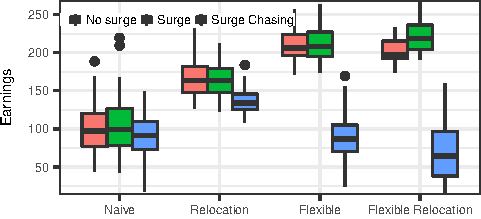
\includegraphics{figures/simulated_earnings.pdf}
	\setlength{\belowcaptionskip}{-10pt}
	\caption{Exploring surge: Simulated earnings for drivers across different strategies on a representative day.}
	\label{fig:simulated_earnings}
\end{figure}

Hence, the question we have to address is the following: 
\textit{Are the conclusions we drew above robust to perturbations of the empirical transition matrices?} We do so using
the framework we developed in Section \ref{sec:sensitivity}:  
we solve the {\robustproblem} problem for each of the four strategies for increasing levels of uncertainty ($\alpha$) using the Sequential Least Squares Programming (SLSQP) minimizer implementation provided by Jones {\etal}~\cite{scipy}.

Figure \ref{fig:uncertainty_evolution} shows the effect of increasing uncertainty on the earnings of drivers for
    each of the four strategies.  We observe two main takeaways.  First, we find that all strategies
   suffer a loss under small amounts of uncertainty, even at levels of $\alpha$ in the range of 0.02, so all
   strategies are tuned closely to the empirical data.  
However, all strategies then remain resilient to a wide range of additional uncertainty, and we find that
   the {\relocation}, {\flexible} and {\relocationflexible} strategies are most tolerant to uncertainty 
  in the input transition matrices. 
Interestingly, even with 99\% uncertainty, the {\relocationflexible} strategy significantly outperforms 
  the {\naive} strategy with no uncertainty.
This observation further supports our claim that being strategic using historical data can significantly improve driver 
  earnings in on-demand ride-hailing platforms. 

\begin{figure}[hb]
	\centering
	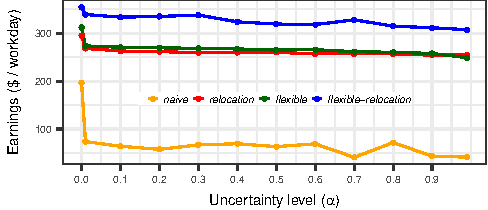
\includegraphics{figures/uncertainty_evolution.pdf}
	\setlength{\belowcaptionskip}{-10pt}
	\caption{Sensitivity to uncertainty in parameters.}
	\label{fig:uncertainty_evolution}
\end{figure}

% \subsection{\textsc{RewardsMatrix}}

% The data gathered in the previous section gives us a matrix of driver earnings, \matr{E}, from passengers while traveling between any two zones in the city. We also get a costs matrix, \matr{C}, whose each entry, $c(i,j) \leq 0$, denotes the sundry expenses of traveling from zone $i$ to zone $j$, dependent on distance and traffic at the given time. The travel costs can result in negative net rewards in the {\gohome} and {\relocate} actions, violating the assumption from Section \ref{sec:problem_setup} that $r(i,j) \geq 0$. In this section, we describe the construction of \textsc{RewardsMatrix}, {\rewardsmatrix}, corresponding to each driver action compliant with our assumptions.

% \subsubsection{\textsc{Modifying the CostsMatrix}}
% If $min\_cost$ is the minimum entry in the matrix \matr{C}, each entry of the modified costs matrix, \matr{C'} is calculated as,
% \begin{equation}
% c'(i,j) = c(i,j) - min\_cost
% \end{equation}
% As a result of the above modification, $\forall i,j : c'(i,j) \geq 0$.

% \subsubsection{\textsc{RewardsMatrix}}
% In order to be compliant with the assumption in Section \ref{sec:problem_setup}, we define two kinds of \textsc{RewardsMatrix}, one for the action {\getpassenger} and another for the actions {\gohome} and {\relocate}.

% \begin{itemize}
% 	\item For the {\getpassenger} action, we define the rewards matrix as,
% 	\begin{equation}
% 		r(i,j) = e(i,j) + c'(i,j) 
% 	\end{equation}
% 	\item For the {\gohome} and {\relocate} actions, the rewards matrix is same as the modified costs matrix.
% 	\begin{equation}
% 		r(i,j) = c'(i,j)
% 	\end{equation}
% \end{itemize}
% In both cases, we set the diagonal entries of the matrix to zero i.e., $\forall i: r(i,i) = 0$.

% It should be noted that this modification does not affect the optimal action choice in any strategy. It merely ensures that the input vectors to the Bisection Algorithm from Section \ref{sec:sensitivity} are always non-negative vectors. Furthermore, while calculating the actual {\totalexpectedearnings} of a driver, we can backtrack these modifications.

% \subsection{\textsc{Comparing robust and nominal strategies}}
% In this section, we compare various strategies. When we choose, $\beta = \betamax$, there is no uncertainty, and we get solution computed via the classical Bellman recursion; referred to as nominal strategy. The robust strategy corresponds to solving the MDP with varying values of $\beta$.

% \subsection{\textsc{Effect of Inaccuracy is uncertainty level}}
% The previous section assumes that, in the robust case, we are able to estimate exactly the precise value of the uncertainty level. In practice, the parameter $\beta$ also has to be estimated. In this section, we study the sensitivity of the robust approach with respect to inaccuracies in the uncertainty parameter $\beta$.
